\chapter{Friedmann Dynamics and the Equation of State}

\lectureoverview{Homogeneous expansion must be separated from local bound physics, and intrinsic geometry must be separated from the shape of an embedding. Once those distinctions are secure, the cosmological principle reduces the spacetime metric to one scale factor \(a(t)\) and one curvature label \(k\). The time-time component of Einstein's equation then becomes the Friedmann energy equation. To solve it we still need the material relation between pressure and energy density. Adiabatic thermodynamics and the equation of state \(P=w\rho\) give \(\rho\propto a^{-3(1+w)}\), unifying matter, radiation, and vacuum energy in one framework.}

\section{Questions That Fix the Physical Picture}

\subsection{Could Space Repeat Before the Horizon?}

A finite flat universe can be represented by a periodic cell. If that cell were smaller than the observable region, light could traverse it and the sky would contain repeated views of the same structures. Detecting those repetitions is harder than simply recognizing a familiar galaxy: the images arrive from different directions and epochs and are altered by cosmic evolution. Nevertheless, periodic topology has observable consequences.

\begin{classroomqa}
\audiencequestion{Could the whole universe be smaller than the observable universe?}
\lecturerresponse{A periodically identified torus is the natural proposal. We would then be observing repeated copies of the same physical region, figuratively seeing ourselves through the back door. Searches for the corresponding cosmic periodicity have not produced supporting evidence and do place constraints on small fundamental cells. The possibility is geometrically consistent, but a universe smaller than the region already observed is not favored by this evidence. \lecturetimestamp{00:01:17--00:02:33}}
\end{classroomqa}

\subsection{Expansion Does Not Pull Apart Bound Systems}

Cosmic expansion describes the large-scale motion of freely moving matter in the average cosmological geometry. It is not a universal command that every proper length must increase. Electromagnetic forces bind atoms, gravity binds planetary systems, and ordinary molecular forces bind solid objects. These interactions are enormously stronger than the cosmological correction on such scales.

\begin{classroomqa}
\audiencequestion{Is the expansion caused by dark energy, and why do atoms or planetary orbits not expand with space?}
\lecturerresponse{The universe was known to expand before dark energy was discovered. Dark energy changes the expansion by accelerating it; it is not the definition or original cause of expansion. A bound system does not follow the Hubble flow because its local forces dominate. An accelerated background can produce an exceedingly small perturbation of an atom or an orbit, but ordinary binding restores an almost unchanged equilibrium rather than allowing the system to fly apart. \lecturetimestamp{00:02:36--00:06:50}}
\end{classroomqa}

\subsection{Energy in a Time-Dependent Geometry}

The remaining objection is not about force but bookkeeping. If a bound orbit continually resists a small cosmological perturbation, where does the required energy come from? The premise imports a conservation law from a static background into a spacetime that has no global time-translation symmetry.

\begin{classroomqa}
\audiencequestion{Where does the energy come from when local binding resists expansion?}
\lecturerresponse{Energy conservation in a static world follows from time-translation invariance: the background and its laws look the same when an experiment is shifted in time. An expanding spacetime is not time-translation invariant in that global sense, so there need not be a single conserved total energy for the entire universe. Local stress-energy conservation still holds and will appear below as the continuity equation. What fails is the naive claim that a globally defined cosmic energy must remain fixed while the geometry changes. \lecturetimestamp{00:06:52--00:09:24}}
\end{classroomqa}

\subsection{Homogeneity Is a Coarse-Grained Statement}

The cosmological principle is scale dependent. Air in a closed room may be nearly uniform on the scale of the room but is granular on molecular scales. The universe likewise contains planets, galaxies, clusters, and density fluctuations. Homogeneity and isotropy refer to its averaged behavior over distances large enough that those structures cease to select a location or direction.

\begin{classroomqa}
\audiencequestion{Do small-scale bound structures contradict homogeneity and isotropy?}
\lecturerresponse{No. Exact homogeneity fails on small scales, just as it fails for air when individual molecules are resolved. On scales of hundreds of millions of light-years and larger, the observed distribution is approximately uniform and direction independent. Beyond the region we can observe, homogeneity remains an assumption whose consequences must be tested rather than an established fact. \lecturetimestamp{00:09:27--00:10:55}}
\end{classroomqa}

\section{Homogeneity and Isotropy as Metric Statements}

Homogeneity and isotropy are geometrical statements before they become dynamical ones. Einstein's equation will tell us how geometry changes with time. First we must say what kind of spatial geometry is allowed at any one time.

\begin{classroomqa}
\audiencequestion{What do homogeneity and isotropy mean mathematically?}
\lecturerresponse{Describe the space by a metric and choose coordinates \(x^i\) centered on one point. Now choose coordinates \(y^i\) centered on another point. Homogeneity means that a transformation can move the origin while leaving the metric with the same functional form. Every point is then geometrically equivalent to every other. Isotropy adds rotational symmetry about each point, so no direction is preferred. \lecturetimestamp{00:11:13--00:14:26}}
\end{classroomqa}

\begin{definition}
A space is \emph{homogeneous} if an isometry can carry any point into any other point. It is \emph{isotropic} about a point if rotations through that point leave its geometry unchanged. A space that is homogeneous and isotropic has neither a preferred position nor a preferred direction.
\end{definition}

The Euclidean plane makes the definition transparent. In Cartesian coordinates,
\begin{equation}
ds^2=dx_1^2+dx_2^2.
\label{eq:c04-flat-metric}
\end{equation}
Move the origin by constants \(a_1\) and \(a_2\):
\begin{equation}
y_1=x_1+a_1,
\qquad
y_2=x_2+a_2.
\label{eq:c04-flat-translation}
\end{equation}
Because \(dy_i=dx_i\), the translated metric is
\begin{equation}
ds^2=dy_1^2+dy_2^2.
\end{equation}
The symbols used to label the point have changed, but the distance rule has not. This is the simplest realization of homogeneity. Rotations likewise preserve the metric, so the plane is isotropic as well. \lecturetimestamp{00:14:27--00:17:30}

The sphere is less trivial only because its coordinates are less convenient. With the south pole chosen as origin, the unit two-sphere can be written
\begin{equation}
d\Omega_2^2=dr^2+\sin^2 r\,d\theta^2.
\label{eq:c04-sphere-metric}
\end{equation}
Rotate the sphere so that an east pole becomes the new origin. The coordinate transformation is cumbersome, but the result is again equation~\eqref{eq:c04-sphere-metric}. No point on a round sphere is geometrically distinguished. \lecturetimestamp{00:17:31--00:20:17}

\begin{classroomqa}
\audiencequestion{Is a periodically identified flat torus both homogeneous and isotropic?}
\lecturerresponse{It is homogeneous under translations: every point in the periodic cell has the same local geometry. It is not fully isotropic, because the identifications pick out preferred periodic directions and lengths. Looking along one of those axes is globally different from looking in a generic oblique direction. The torus therefore supplies a clean example of homogeneity without complete isotropy. \lecturetimestamp{00:20:18--00:21:30}}
\end{classroomqa}

Observed large-scale uniformity motivates the cosmological principle within our horizon. Extending it beyond the observable region is a postulate, not a direct observation. We accept that postulate because it gives a sharply defined geometry whose consequences can be confronted with data. \lecturetimestamp{00:21:43--00:22:12}

\section{Intrinsic Geometry and Embedding}

When space is called spherical, it is tempting to imagine the rubber surface of a balloon placed inside a larger room. That picture may help us draw, but the surrounding room is not part of the cosmological assertion. The geometry that matters is \emph{intrinsic}: it consists of distances and angles measurable by observers who remain within the space. \lecturetimestamp{00:22:13--00:23:19}

\subsection{Closed One-Dimensional Worlds}

Consider a closed one-dimensional world. We may draw it as a circle, a square with rounded corners, or a peanut-shaped loop. An inhabitant confined to the line measures only distance along it. If two loops have the same total circumference, then those inhabitants encounter the same intrinsic geometry even when the drawings look entirely different.

\begin{figure}[htbp]
\centering

\includegraphics[width=0.72\textwidth]{lecture_04_figure_05.png}
\caption{Round and deformed closed loops used to distinguish intrinsic geometry from embedding shape. This later frame preserves drawings made during the earlier discussion; the relevant content occurs at 00:23:21--00:25:59.}
\label{fig:c04-intrinsic-board}
\lectureframe{00:59:54.899}
\end{figure}

Every one-dimensional metric is locally flat. A short piece of string can be straightened without stretching it, so visible bending in the surrounding plane is extrinsic rather than intrinsic curvature. A closed loop has a global modulus, its circumference, but it has no intrinsic local bending that its one-dimensional inhabitants can measure. \lecturetimestamp{00:23:21--00:25:59}

\begin{figure}[htbp]
\centering
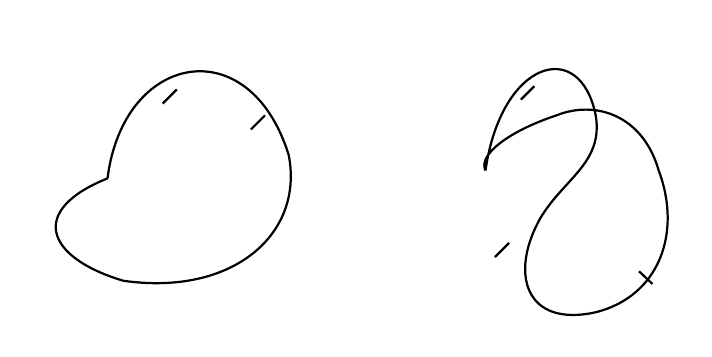
\begin{tikzpicture}[scale=1.0]
\draw[line width=0.8pt] (0,0)
  .. controls (0.2,1.6) and (1.8,1.9) .. (2.3,0.3)
  .. controls (2.5,-0.7) and (1.6,-1.5) .. (0.2,-1.3)
  .. controls (-0.8,-1.0) and (-1.0,-0.4) .. (0,0);
\draw[line width=0.8pt] (0.70,0.95) -- (0.88,1.13);
\draw[line width=0.8pt] (1.82,0.62) -- (2.00,0.80);

\draw[line width=0.8pt] (4.8,0.1)
  .. controls (5.0,1.5) and (6.0,1.8) .. (6.2,0.8)
  .. controls (6.3,0.2) and (5.8,0.0) .. (5.5,-0.5)
  .. controls (5.1,-1.2) and (5.3,-1.9) .. (6.2,-1.7)
  .. controls (7.0,-1.5) and (7.3,-0.7) .. (7.0,0.1)
  .. controls (6.8,0.8) and (6.2,1.0) .. (5.7,0.8)
  .. controls (5.1,0.6) and (4.7,0.3) .. (4.8,0.1);
\draw[line width=0.8pt] (5.25,1.00) -- (5.42,1.17);
\draw[line width=0.8pt] (5.10,-0.82) -- (4.92,-1.00);
\draw[line width=0.8pt] (6.75,-1.18) -- (6.92,-1.34);
\end{tikzpicture}
\caption{A clean reconstruction of the circle and deformed loop. Equal circumference means equal intrinsic one-dimensional geometry.}
\label{fig:c04-intrinsic-redraw}
\end{figure}

\begin{classroomqa}
\audiencequestion{Would a finite line segment be the same kind of one-dimensional space?}
\lecturerresponse{No. A segment has two endpoints, whereas a closed loop has none. That topological distinction is intrinsic and cannot be removed by bending either object in a larger space. Once the topology is fixed, the segment is characterized by its length and the closed loop by its circumference. \lecturetimestamp{00:26:00--00:26:39}}
\end{classroomqa}

\subsection{Why Embeddings Are Useful but Optional}

We visualize a one-dimensional circle by placing it in two dimensions and a two-dimensional sphere by placing it in three. The pattern tempts us to demand a fourth Euclidean dimension before discussing a three-sphere. That demand reflects human visualization, not a mathematical necessity. Our visual machinery evolved to navigate three dimensions; coordinates and metrics let us reason beyond that limit without constructing a literal external viewpoint. \lecturetimestamp{00:26:40--00:29:54}

\begin{classroomqa}
\audiencequestion{Could additional spatial dimensions exist but be too small to see?}
\lecturerresponse{Yes. Geometry does not require all dimensions to have the same observable extent. A compact dimension could be much smaller than the scales probed by ordinary experience. The immediate point, however, is simpler: whether or not extra dimensions exist physically, an embedding dimension is unnecessary for defining the intrinsic metric of our three-dimensional space. \lecturetimestamp{00:29:55--00:30:12}}
\end{classroomqa}

\begin{classroomqa}
\audiencequestion{How would an inhabitant confined to a curved line know whether the line is bent?}
\lecturerresponse{It could not know from intrinsic measurements alone. Imagine light and matter confined to an optical fiber. Bending the fiber without stretching it changes the embedding but not the distances or signal travel times measured along the fiber. Only a signal that escaped into the surrounding space could reveal the external bend. \lecturetimestamp{00:30:15--00:31:14}}
\end{classroomqa}

The thought experiment can be made operational. A creature restricted to the fiber could launch a signal, such as a sufficiently energetic photon, and discover an external direction only if the signal escaped the fiber and later returned by a route unavailable within the one-dimensional metric. In the same spirit, the statement that ordinary space has three large dimensions is ultimately experimental, not a deduction from what the human mind can picture. \lecturetimestamp{00:32:31--00:33:42}

\begin{classroomqa}
\audiencequestion{If every one-dimensional space is locally flat, is every two-dimensional space locally flat as well?}
\lecturerresponse{No. A sheet rolled into a cylinder remains intrinsically flat because it can be unrolled without stretching. A hemisphere cannot be flattened onto a plane without stretching or tearing, so it possesses intrinsic curvature. A sufficiently small patch always looks approximately Euclidean, but measurable deviations appear at finite scale. The distinction between a cylinder and a sphere is exactly the distinction between extrinsic bending and intrinsic curvature. \lecturetimestamp{00:31:14--00:35:00}}
\end{classroomqa}

\begin{classroomqa}
\audiencequestion{Does intrinsic curvature necessarily mean that a gravitational field is present?}
\lecturerresponse{In general relativity, spacetime curvature is the invariant manifestation of tidal gravity. The cosmological spatial curvature \(k/a^2\) is therefore part of the gravitational geometry, not merely a bend in an imagined external space. Matter influences curvature through Einstein's equation, but one should not sharpen the statement into "curvature exists only where matter sits": vacuum spacetime can carry Weyl curvature, as outside a star or in a gravitational wave. \lecturetimestamp{00:35:01--00:35:51}}
\end{classroomqa}

We now impose the large-scale idealization. Average over stars, galaxies, clusters, and local irregularities, just as one ignores mountains when describing Earth as round. The resulting spatial geometry is taken to be homogeneous and isotropic. Under these assumptions there are three constant-curvature possibilities: flat, spherical, and hyperbolic. \lecturetimestamp{00:36:08--00:38:44}

\section{The FRW Ansatz and the Three Curvature Cases}

The symmetry assumptions collapse the geometry to one time-dependent scale and one discrete curvature sign. In comoving coordinates the Friedmann-Robertson-Walker ansatz is
\begin{equation}
ds^2=-dt^2+a(t)^2\,d\Sigma_k^2,
\qquad
k\in\{-1,0,+1\}.
\label{eq:c04-frw}
\end{equation}
The time coordinate is the proper time of comoving observers. Homogeneity permits \(a\) to depend on time but not position, while isotropy forbids a preferred spatial direction. \lecturetimestamp{00:38:46--00:40:22}

\begin{figure}[htbp]
\centering

\includegraphics[width=0.74\textwidth]{lecture_04_figure_02.png}
\caption{The three constant-curvature spatial metrics grouped beneath the common scale factor. The frame was captured later, after the board had accumulated other material, but it preserves the metric discussion from 00:40:23--00:42:42.}
\label{fig:c04-frw-board}
\lectureframe{00:45:48.386}
\end{figure}

Using a radial coordinate \(r\) and the unit two-sphere metric \(d\Omega_2^2\), the three normalized spatial metrics are
\begin{align}
d\Sigma_0^2 &= dr^2+r^2d\Omega_2^2,
&& k=0,
\label{eq:c04-flat-space}\\
d\Sigma_{+1}^2 &= dr^2+\sin^2 r\,d\Omega_2^2,
&& k=+1,
\label{eq:c04-spherical-space}\\
d\Sigma_{-1}^2 &= dr^2+\sinh^2 r\,d\Omega_2^2,
&& k=-1.
\label{eq:c04-hyperbolic-space}
\end{align}
At a fixed time, space is therefore flat, positively curved, or negatively curved. Multiplication by \(a(t)^2\) changes every spatial distance by the same factor while preserving the normalized shape. \lecturetimestamp{00:40:23--00:42:42}

Take two galaxies at fixed comoving separation \(\Delta\chi\). Their physical distance is
\begin{equation}
D(t)=a(t)\Delta\chi.
\end{equation}
Differentiating and eliminating \(\Delta\chi\) gives
\begin{equation}
\dot D=\dot a\,\Delta\chi
      =\frac{\dot a}{a}D
      =H(t)D,
\qquad
H(t)\equiv\frac{\dot a}{a}.
\label{eq:c04-hubble-law}
\end{equation}
Thus Hubble's law follows kinematically from homogeneous scaling. The Hubble parameter can change with time, but at any fixed cosmic time it is the same everywhere. \lecturetimestamp{00:42:45--00:44:23}

\section{From Einstein's Equation to Friedmann's Equation}

The metric tells us how distances are measured, but not how \(a(t)\) evolves. Curved spacetime requires Einstein's equation. Computing every Christoffel symbol and curvature component would obscure the physical argument, so we use the form forced by symmetry and isolate its time-time component. \lecturetimestamp{00:44:25--00:46:33}

In units with \(c=1\) and with a cosmological constant temporarily omitted, the full tensor equation is
\begin{equation}
G_{\mu\nu}
\equiv
R_{\mu\nu}-\frac12 g_{\mu\nu}R
=8\pi G\,T_{\mu\nu}.
\label{eq:c04-einstein}
\end{equation}
Geometry occupies the left-hand side; energy density, momentum density, pressure, and stress occupy the right. The factor \(1/3\) does not belong in the full tensor equation. It appears only after the time-time component has been reduced to Friedmann form.

\begin{figure}[htbp]
\centering

\includegraphics[width=0.78\textwidth]{lecture_04_figure_03.png}
\caption{An intermediate board state of Einstein's equation. The geometric left-hand side is visible, while the matter tensor is not yet legible and the displayed normalization is incomplete. Equation~\eqref{eq:c04-einstein} records the standard completed tensor equation used in the derivation.}
\label{fig:c04-einstein-board}
\lectureframe{00:48:19.394}
\end{figure}

For a homogeneous fluid at rest in comoving coordinates,
\begin{equation}
T_{00}=\rho.
\label{eq:c04-energy-density}
\end{equation}
The time-time Einstein tensor has a useful structural property. Its second derivatives cancel, leaving one term quadratic in the first time derivative and one term from spatial curvature:
\begin{equation}
G_{00}=3\left[
\left(\frac{\dot a}{a}\right)^2+\frac{k}{a^2}
\right].
\label{eq:c04-g00}
\end{equation}
Substituting equations~\eqref{eq:c04-energy-density} and \eqref{eq:c04-g00} into equation~\eqref{eq:c04-einstein} gives the first Friedmann equation,
\begin{equation}
\boxed{
\left(\frac{\dot a}{a}\right)^2+\frac{k}{a^2}
=\frac{8\pi G}{3}\rho
}.
\label{eq:c04-friedmann}
\end{equation}
Equivalently,
\begin{equation}
H^2=\frac{8\pi G}{3}\rho-\frac{k}{a^2}.
\label{eq:c04-friedmann-energy}
\end{equation}
\lecturetimestamp{00:46:33--00:55:53}

Equation~\eqref{eq:c04-friedmann-energy} has exactly the form found in the earlier Newtonian argument. There the integration constant was interpreted as the total mechanical energy or escape condition of a sphere of matter. General relativity places intrinsic spatial curvature in the same mathematical slot. The agreement is not an accident: in a sufficiently small region, curvature effects become negligible and relativistic cosmology must reproduce local Newtonian behavior. Relativity also clarifies that \(\rho\) means total energy density, so relativistic particles and photons gravitate even though a nonrelativistic mass-density argument would miss them. \lecturetimestamp{00:55:55--00:58:23}

\begin{classroomqa}
\audiencequestion{Why are there no terms mixing space and time in the metric?}
\lecturerresponse{A mixed term would behave like a preferred spatial vector or flow relative to the comoving observers. Exact homogeneity and isotropy leave no such direction available. In coordinates adapted to the cosmic matter, the shift therefore vanishes and the metric takes the block-diagonal form in equation~\eqref{eq:c04-frw}. If the assumed symmetries are preserved, this is not an extra dynamical guess but their geometrical consequence. \lecturetimestamp{00:58:27--00:59:08}}
\end{classroomqa}

\begin{classroomqa}
\audiencequestion{Why is the time-time component enough, and where did the second derivatives go?}
\lecturerresponse{The homogeneous and isotropic ansatz contains only one unknown function, \(a(t)\). The mixed components reduce to identities, while the spatial components are related to the time-time equation and stress-energy conservation. One may combine them into an acceleration equation containing \(\ddot a\), but the time-time Einstein tensor is special: its second-derivative terms cancel, leaving the first-order energy equation~\eqref{eq:c04-friedmann}. One nontrivial equation plus the material evolution law is enough to determine the single geometric degree of freedom. \lecturetimestamp{00:59:09--01:00:56}}
\end{classroomqa}

\section{How the Contents of the Universe Dilute}

Friedmann's equation is not closed until \(\rho\) is known as a function of \(a\). Geometry has supplied one equation; the material in the universe must supply the second relation. \lecturetimestamp{01:01:05--01:02:34}

For nonrelativistic matter, the number of particles in a comoving volume is fixed while the physical volume grows as \(a^3\). Neglecting the particles' small kinetic energies,
\begin{equation}
\rho_{\mathrm m}(a)=\frac{\rho_{\mathrm m,0}}{a^3}.
\label{eq:c04-matter-scaling}
\end{equation}
Here the normalization \(a=1\) may be assigned at any convenient reference epoch; only ratios of scale factors are directly meaningful. \lecturetimestamp{01:02:35--01:05:02}

\begin{classroomqa}
\audiencequestion{If a flat universe is infinite, what does it mean for \(a\) to shrink toward the big bang?}
\lecturerresponse{An infinite flat space remains infinite for every nonzero value of \(a\); all finite comoving separations are multiplied by the same shrinking factor. The absolute normalization of \(a\) is arbitrary in the flat case, so only \(a(t_2)/a(t_1)\) has invariant meaning. For a closed spherical universe \(a\) is naturally its curvature radius, and for a hyperbolic universe it sets the curvature radius. The limit \(a\to0\) signals the cosmological singularity, not an ordinary finite ball sitting in external space. \lecturetimestamp{01:05:06--01:05:53}}
\end{classroomqa}

Radiation loses energy in two ways. Its number density falls as the inverse volume, and every photon's wavelength stretches in proportion to \(a\), reducing its energy by another factor of \(a^{-1}\). Therefore
\begin{equation}
\rho_{\mathrm r}(a)=\frac{\rho_{\mathrm r,0}}{a^4}.
\label{eq:c04-radiation-scaling}
\end{equation}
Because \(a^{-4}\) grows faster toward the past than \(a^{-3}\), radiation dominates sufficiently early even if matter dominates much later. \lecturetimestamp{01:05:54--01:06:45}

If matter and radiation were the only components, the sign of \(k\) would strongly track the future: \(k=+1\) permits recollapse, \(k=0\) is the marginal case that expands forever while slowing, and \(k=-1\) expands forever with curvature eventually important. Dark energy breaks that simple connection. A closed universe can expand forever, and spatial flatness by itself does not determine the ultimate fate. \lecturetimestamp{01:06:45--01:08:10}

\section{Equation of State and the Continuity Law}

Rather than memorize a separate dilution rule for every substance, characterize the material by an equation of state. The program has two parts. First derive \(\rho(a)\) for a given relation between pressure and energy density. Then determine that relation from the microscopic physics of matter, radiation, or vacuum. The first part is enough for the present lecture. \lecturetimestamp{01:08:19--01:11:00}

Pressure is momentum flux. Molecules striking the wall of a box reverse their momentum and push on the wall; faster particles transfer more momentum and produce greater pressure. Energy density and pressure therefore cannot be chosen independently once the kind of material is specified. For a simple cosmological component we write
\begin{equation}
P=w\rho,
\label{eq:c04-equation-state}
\end{equation}
where \(w\) is dimensionless in units with \(c=1\). Cold matter has negligible pressure and hence \(w=0\). Radiation has \(w=1/3\), with the factor \(1/3\) reflecting the average over three spatial directions. \lecturetimestamp{01:11:00--01:16:34}

\begin{figure}[htbp]
\centering

\includegraphics[width=0.82\textwidth]{lecture_04_figure_06.png}
\caption{The board collects the matter and radiation scalings and writes the equation of state as \(P=W\rho\). We use the conventional lowercase \(w\).}
\label{fig:c04-equation-state-board}
\lectureframe{01:15:08.166}
\end{figure}

\subsection{Thermodynamics in a Comoving Box}

Take a comoving box with physical volume \(V\), energy density \(\rho\), and total energy
\begin{equation}
E=\rho V.
\end{equation}
The first law is
\begin{equation}
dE=T\,dS-P\,dV.
\end{equation}
Cosmological expansion is treated as adiabatic, so \(dS=0\) for the comoving box and
\begin{equation}
dE=-P\,dV.
\label{eq:c04-adiabatic-first-law}
\end{equation}
The minus sign says that an expanding system does work and loses internal energy. Differentiating \(E=\rho V\) independently gives
\begin{equation}
dE=\rho\,dV+V\,d\rho.
\end{equation}
Equating the two expressions,
\begin{align}
\rho\,dV+V\,d\rho&=-P\,dV,\\
V\,d\rho&=-(\rho+P)\,dV.
\label{eq:c04-volume-continuity}
\end{align}
With \(P=w\rho\),
\begin{equation}
\frac{d\rho}{\rho}=-(1+w)\frac{dV}{V}.
\end{equation}
Integration gives
\begin{equation}
\rho\propto V^{-(1+w)}.
\end{equation}
Since a comoving volume scales as \(V\propto a^3\),
\begin{equation}
\boxed{\rho(a)\propto a^{-3(1+w)}}.
\label{eq:c04-density-scaling}
\end{equation}
In differential form, the same statement is the local energy-conservation equation
\begin{equation}
\dot\rho+3H(\rho+P)=0.
\label{eq:c04-continuity}
\end{equation}
This local conservation law remains exact even though a changing cosmological geometry need not admit a globally conserved total energy. \lecturetimestamp{01:16:35--01:25:30}

The two familiar cases follow immediately:
\begin{align}
w=0
&\quad\Longrightarrow\quad
\rho_{\mathrm m}\propto a^{-3},\\
w=\frac13
&\quad\Longrightarrow\quad
\rho_{\mathrm r}\propto a^{-4}.
\end{align}
The extra inverse power for radiation is the thermodynamic expression of cosmological redshift. \lecturetimestamp{01:25:31--01:26:40}

\begin{classroomqa}
\audiencequestion{What radiation remains in the universe today?}
\lecturerresponse{The classroom discussion points chiefly to the cosmic microwave background, the relic photon bath from the hot early universe. Radiation is now a small part of the total cosmic energy density, but its \(a^{-4}\) scaling means that it overtakes matter when the equations are run far enough backward. The precise present fractions are observational inputs and are not needed for this scaling argument. \lecturetimestamp{01:26:53--01:28:34}}
\end{classroomqa}

\section{Vacuum Energy and the Failure of the Curvature-Fate Rule}

Dark energy introduces the equation of state
\begin{equation}
P=-\rho,
\qquad
w=-1.
\label{eq:c04-vacuum-eos}
\end{equation}
Negative pressure is tension: instead of pushing outward on the wall of a box, the contents pull inward on it. A stretched spring is a familiar object with tension, though it is only an analogy and not a microscopic model of vacuum energy. \lecturetimestamp{01:28:35--01:31:46}

\begin{classroomqa}
\audiencequestion{Is negative pressure connected with absolute zero?}
\lecturerresponse{Not in any simple general way. Cooling an ordinary material to zero temperature does not by itself produce the cosmological equation of state \(P=-\rho\). The exchange is useful because it distinguishes thermal pressure from vacuum stress: vacuum energy is characterized by Lorentz-invariant stress-energy, whose spatial components act as negative pressure. Its microscopic origin is a separate question. \lecturetimestamp{01:31:01--01:31:46}}
\end{classroomqa}

Substituting \(w=-1\) into equation~\eqref{eq:c04-density-scaling} gives
\begin{equation}
\rho_\Lambda\propto a^0=\text{constant}.
\label{eq:c04-vacuum-density}
\end{equation}
As a comoving region expands, its volume and total vacuum energy increase together, leaving the energy per unit volume unchanged. The work term in equation~\eqref{eq:c04-adiabatic-first-law} accounts for that behavior because \(P\) is negative. Once such a component is present, positive spatial curvature no longer guarantees recollapse. \lecturetimestamp{01:31:57--01:33:29}

\begin{classroomqa}
\audiencequestion{Where do dark matter, black holes, and other compact objects enter?}
\lecturerresponse{On scales large compared with their separations, any nonrelativistic component whose random velocities are small is part of the pressureless matter density. That includes ordinary matter, cold dark matter, and a population of compact objects such as black holes. Their local structure is complicated, but after coarse-graining their average cosmological equation of state is approximately \(w=0\). \lecturetimestamp{01:33:34--01:34:10}}
\end{classroomqa}

\begin{classroomqa}
\audiencequestion{Do the relativistic equations reproduce the matter- and radiation-dominated solutions found earlier?}
\lecturerresponse{Yes. For \(k=0\), inserting \(\rho_{\mathrm m}\propto a^{-3}\) into Friedmann's equation gives \(\dot a^2\propto a^{-1}\) and therefore \(a(t)\propto t^{2/3}\). Inserting \(\rho_{\mathrm r}\propto a^{-4}\) gives \(\dot a^2\propto a^{-2}\) and \(a(t)\propto t^{1/2}\). General relativity changes the interpretation and enlarges the possible sources, but it preserves those solutions. \lecturetimestamp{01:34:14--01:35:12}}
\end{classroomqa}

\begin{classroomqa}
\audiencequestion{What sort of force would dark energy resemble in a Newtonian picture?}
\lecturerresponse{A positive cosmological constant produces a repulsive relative acceleration proportional to separation,
\[
\ddot D=\frac{\Lambda}{3}D
\]
in units with \(c=1\). A negative cosmological constant reverses the sign and is attractive. Because the positive-\(\Lambda\) effect grows with distance, it can eventually dominate matter and curvature; even a closed \(k=+1\) universe can then continue expanding. This Newtonian form is only a useful shadow of the relativistic dynamics. \lecturetimestamp{01:35:13--01:36:55}}
\end{classroomqa}

\section{What to Carry Forward}

The cosmological principle is an averaged geometrical assertion: every point and direction is equivalent after local structure is smoothed away. It restricts the spatial metric to the three constant-curvature cases and packages all time dependence into \(a(t)\):
\begin{equation}
ds^2=-dt^2+a(t)^2d\Sigma_k^2.
\end{equation}
Comoving separations then obey \(\dot D=HD\), while bound systems need not join that flow.

Einstein's time-time equation turns the ansatz into dynamics:
\begin{equation}
H^2+\frac{k}{a^2}=\frac{8\pi G}{3}\rho.
\end{equation}
Its resemblance to the Newtonian energy equation is real, but general relativity identifies the integration slot with intrinsic spatial curvature and allows every form of energy to contribute.

The remaining input is thermodynamic. For an adiabatically expanding component with \(P=w\rho\),
\begin{equation}
\dot\rho+3H(\rho+P)=0,
\qquad
\rho\propto a^{-3(1+w)}.
\end{equation}
Matter, radiation, and vacuum energy correspond respectively to
\begin{equation}
w=0,\qquad w=\frac13,\qquad w=-1.
\end{equation}
Their different dilution rates determine which component controls the expansion at each epoch. The next task is to understand the physics behind these equations of state and the acceleration produced by vacuum energy.
